\documentclass[tikz,border=14pt]{standalone}
\usepackage[T1]{fontenc}
\usepackage[utf8]{inputenc}
\usepackage{helvet}
\renewcommand{\familydefault}{\sfdefault}
\usetikzlibrary{arrows.meta,positioning,calc,backgrounds,fit}

\definecolor{ich}{HTML}{D9602B}
\definecolor{ichhell}{HTML}{FBE9DF}
\definecolor{ki}{HTML}{2F5D8A}
\definecolor{kihell}{HTML}{E6EEF6}
\definecolor{ol}{HTML}{3C8D5A}
\definecolor{olhell}{HTML}{E4F2E9}
\definecolor{rr}{HTML}{6B4FA0}
\definecolor{rrhell}{HTML}{EEE9F6}
\definecolor{db}{HTML}{8A6A2E}
\definecolor{dbhell}{HTML}{F6F0E2}
\definecolor{grau}{HTML}{5A5F66}
\definecolor{bahn}{HTML}{F5F6F8}

\begin{document}
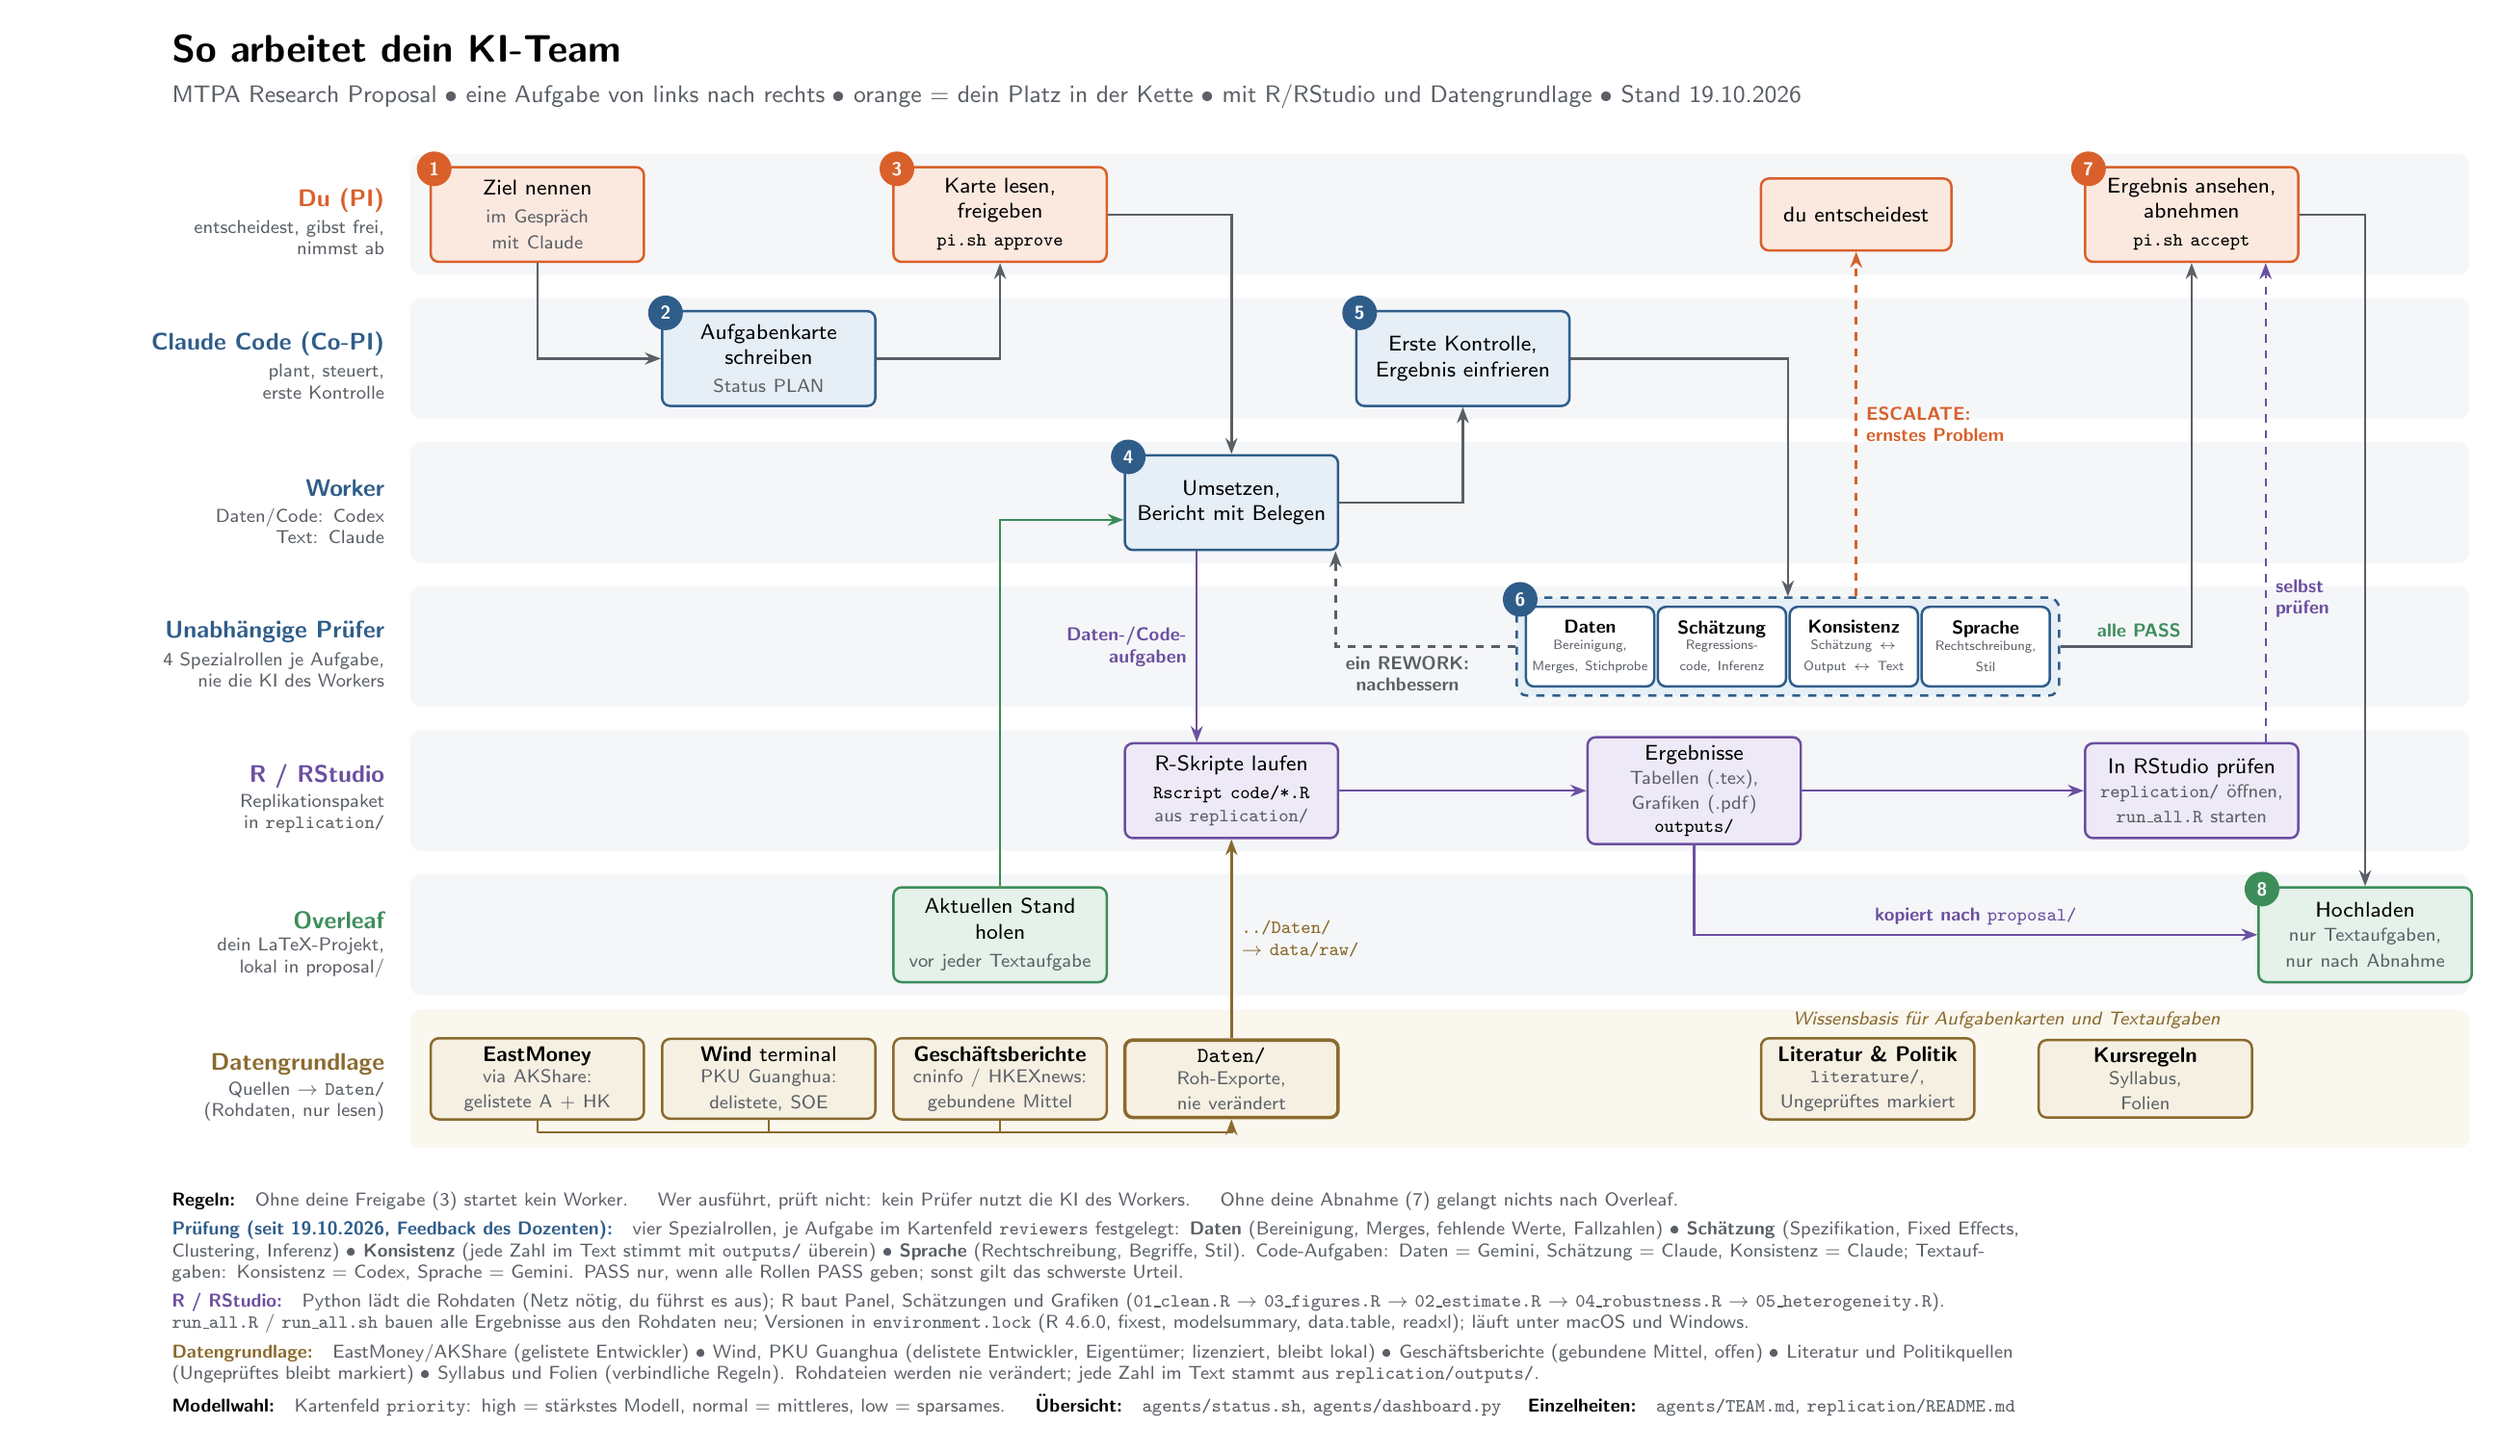
\begin{tikzpicture}[
  x=3.05cm, y=1.9cm,
  kasten/.style={rounded corners=3pt, draw=#1, line width=0.9pt, align=center,
                 text width=2.6cm, minimum height=1.25cm, font=\footnotesize, inner sep=3pt},
  ich/.style={kasten=ich, fill=ichhell},
  ki/.style={kasten=ki, fill=kihell},
  ol/.style={kasten=ol, fill=olhell},
  rr/.style={kasten=rr, fill=rrhell},
  db/.style={kasten=db, fill=dbhell, minimum height=1.0cm},
  rv/.style={kasten=ki, fill=white, text width=1.55cm, minimum height=1.05cm, font=\scriptsize, inner sep=2pt},
  pfeil/.style={-{Stealth[length=6pt]}, line width=0.9pt, draw=grau},
  lbl/.style={font=\scriptsize\bfseries, text=#1},
  nr/.style={circle, fill=#1, text=white, font=\scriptsize\bfseries, inner sep=1.3pt, minimum size=13pt},
  bahnname/.style={font=\small\bfseries, anchor=east, align=right, text width=4.6cm},
  bahnsub/.style={font=\scriptsize, text=grau, anchor=east, align=right, text width=4.6cm},
]

% ---------------------------------------------------------------- lanes
\begin{scope}[on background layer]
  \foreach \y in {6,5,4,3,2,1} {
    \fill[bahn, rounded corners=4pt] (0.45,\y-0.42) rectangle (9.35,\y+0.42);
  }
  \fill[dbhell!55, rounded corners=4pt] (0.45,-0.48) rectangle (9.35,0.48);
\end{scope}

\node[bahnname, text=ich] at (0.38,6.10) {Du (PI)};
\node[bahnsub]            at (0.38,5.84) {entscheidest, gibst frei,\\nimmst ab};
\node[bahnname, text=ki]  at (0.38,5.10) {Claude Code (Co-PI)};
\node[bahnsub]            at (0.38,4.84) {plant, steuert,\\erste Kontrolle};
\node[bahnname, text=ki]  at (0.38,4.10) {Worker};
\node[bahnsub]            at (0.38,3.84) {Daten/Code: Codex\\Text: Claude};
\node[bahnname, text=ki]  at (0.38,3.10) {Unabh\"angige Pr\"ufer};
\node[bahnsub]            at (0.38,2.84) {4 Spezialrollen je Aufgabe,\\nie die KI des Workers};
\node[bahnname, text=rr]  at (0.38,2.10) {R / RStudio};
\node[bahnsub]            at (0.38,1.84) {Replikationspaket\\in \texttt{replication/}};
\node[bahnname, text=ol]  at (0.38,1.10) {Overleaf};
\node[bahnsub]            at (0.38,0.84) {dein LaTeX-Projekt,\\lokal in proposal/};
\node[bahnname, text=db]  at (0.38,0.10) {Datengrundlage};
\node[bahnsub]            at (0.38,-0.16) {Quellen $\rightarrow$ \texttt{Daten/}\\(Rohdaten, nur lesen)};

% ---------------------------------------------------------------- task steps
\node[ich] (s1) at (1,6) {Ziel nennen\\[1pt]{\scriptsize\color{grau}im Gespr\"ach mit Claude}};
\node[ki]  (s2) at (2,5) {Aufgabenkarte schreiben\\[1pt]{\scriptsize\color{grau}Status PLAN}};
\node[ich] (s3) at (3,6) {Karte lesen,\\freigeben\\[1pt]{\scriptsize\ttfamily pi.sh approve}};
\node[ki]  (s4) at (4,4) {Umsetzen,\\Bericht mit Belegen};
\node[ki]  (s5) at (5,5) {Erste Kontrolle,\\Ergebnis einfrieren};
% four specialised reviewers (since 19 Oct 2026)
\node[rv] (v1) at (5.55,3) {\textbf{Daten}\\[0pt]{\tiny\color{grau}Bereinigung,\\Merges, Stichprobe}};
\node[rv] (v2) at (6.12,3) {\textbf{Sch\"atzung}\\[0pt]{\tiny\color{grau}Regressions-\\code, Inferenz}};
\node[rv] (v3) at (6.69,3) {\textbf{Konsistenz}\\[0pt]{\tiny\color{grau}Sch\"atzung $\leftrightarrow$\\Output $\leftrightarrow$ Text}};
\node[rv] (v4) at (7.26,3) {\textbf{Sprache}\\[0pt]{\tiny\color{grau}Rechtschreibung,\\Stil}};
\node[draw=ki, line width=0.9pt, dashed, rounded corners=4pt, fit=(v1)(v4), inner sep=3pt] (s6) {};
\begin{scope}[on background layer]\node[fill=kihell, rounded corners=4pt, fit=(v1)(v4), inner sep=3pt] {};\end{scope}
\node[ich] (s7) at (8.15,6) {Ergebnis ansehen,\\abnehmen\\[1pt]{\scriptsize\ttfamily pi.sh accept}};
\node[ol]  (s8) at (8.9,1) {Hochladen\\[1pt]{\scriptsize\color{grau}\mbox{nur Textaufgaben,}\\\mbox{nur nach Abnahme}}};
\node[ol]  (p4) at (3,1) {Aktuellen Stand\\holen\\[1pt]{\scriptsize\color{grau}\mbox{vor jeder Textaufgabe}}};
\node[ich, text width=2.3cm, minimum height=0.95cm] (esc) at (6.7,6) {\mbox{du entscheidest}};

% ---------------------------------------------------------------- R / RStudio lane
\node[rr] (r1) at (4,2) {R-Skripte laufen\\[1pt]{\scriptsize\ttfamily Rscript code/*.R}\\[-1pt]{\scriptsize\color{grau}aus \texttt{replication/}}};
\node[rr] (r2) at (6.0,2) {Ergebnisse\\[1pt]{\scriptsize\color{grau}\mbox{Tabellen (.tex),}\\\mbox{Grafiken (.pdf)}}\\[-1pt]{\scriptsize\ttfamily outputs/}};
\node[rr] (r3) at (8.15,2) {In RStudio pr\"ufen\\[1pt]{\scriptsize\color{grau}\mbox{\texttt{replication/} \"offnen,}\\\mbox{\texttt{run\_all.R} starten}}};

% ---------------------------------------------------------------- data basis lane
\node[db] (d1) at (1,0) {\textbf{EastMoney}\\[0pt]{\scriptsize\color{grau}\mbox{via AKShare:}\\\mbox{gelistete A + HK}}};
\node[db] (d2) at (2,0) {\textbf{Wind} terminal\\[0pt]{\scriptsize\color{grau}\mbox{PKU Guanghua:}\\\mbox{delistete, SOE}}};
\node[db] (d3) at (3,0) {\textbf{Gesch\"aftsberichte}\\[0pt]{\scriptsize\color{grau}\mbox{cninfo / HKEXnews:}\\\mbox{gebundene Mittel}}};
\node[db, line width=1.3pt] (dD) at (4,0) {\texttt{Daten/}\\[0pt]{\scriptsize\color{grau}\mbox{Roh-Exporte,}\\\mbox{nie ver\"andert}}};
\node[db] (d4) at (6.75,0) {\textbf{Literatur \& Politik}\\[0pt]{\scriptsize\color{grau}\mbox{\texttt{literature/},}\\\mbox{Ungepr\"uftes markiert}}};
\node[db] (d5) at (7.95,0) {\textbf{Kursregeln}\\[0pt]{\scriptsize\color{grau}\mbox{Syllabus,}\\\mbox{Folien}}};

% numbers
\node[nr=ich] at ($(s1.north west)+(0.02,-0.02)$) {1};
\node[nr=ki]  at ($(s2.north west)+(0.02,-0.02)$) {2};
\node[nr=ich] at ($(s3.north west)+(0.02,-0.02)$) {3};
\node[nr=ki]  at ($(s4.north west)+(0.02,-0.02)$) {4};
\node[nr=ki]  at ($(s5.north west)+(0.02,-0.02)$) {5};
\node[nr=ki]  at ($(s6.north west)+(0.02,-0.02)$) {6};
\node[nr=ich] at ($(s7.north west)+(0.02,-0.02)$) {7};
\node[nr=ol]  at ($(s8.north west)+(0.02,-0.02)$) {8};

% ---------------------------------------------------------------- main flow
\draw[pfeil] (s1.south) |- (s2.west);
\draw[pfeil] (s2.east) -| (s3.south);
\draw[pfeil] (s3.east) -| (s4.north);
\draw[pfeil] (s4.east) -| (s5.south);
\draw[pfeil] (s5.east) -| (s6.north);
\draw[pfeil] (s6.east) -| node[pos=0.3, above, lbl=ol] {alle PASS} (s7.south);
\draw[pfeil] (s7.east) -| (s8.north);
\draw[pfeil, draw=ol] (p4.north) |- ($(s4.west)+(0,-0.12)$);

% loops
\draw[pfeil, dashed] (s6.west) -| node[pos=0.3, below, lbl=grau, align=center] {ein REWORK:\\nachbessern} ($(s4.south)+(0.45,0)$);
\draw[pfeil, dashed, draw=ich] (s6.north -| esc.south) -- node[pos=0.5, right, lbl=ich, align=left] {ESCALATE:\\ernstes Problem} (esc.south);

% ---------------------------------------------------------------- R connections
\draw[pfeil, draw=rr] ($(s4.south)+(-0.15,0)$) -- node[pos=0.5, left, lbl=rr, align=right] {Daten-/Code-\\aufgaben} ($(r1.north)+(-0.15,0)$);
\draw[pfeil, draw=rr] (r1.east) -- (r2.west);
\draw[pfeil, draw=rr] (r2.east) -- (r3.west);
\draw[pfeil, draw=rr, dashed] ($(r3.north)+(0.32,0)$) -- node[pos=0.3, right, lbl=rr, align=left] {selbst\\pr\"ufen} ($(s7.south)+(0.32,0)$);
\draw[pfeil, draw=rr] (r2.south) |- node[pos=0.75, above, lbl=rr] {kopiert nach \texttt{proposal/}} (s8.west);

% ---------------------------------------------------------------- data basis connections
\node[font=\scriptsize\itshape, text=db] at ($(d4.north)!0.5!(d5.north)+(0,0.12)$) {Wissensbasis f\"ur Aufgabenkarten und Textaufgaben};
\coordinate (bus) at (0,-0.37);
\foreach \d in {d1,d2,d3} { \draw[line width=0.9pt, draw=db] (\d.south) -- (\d.south |- bus); }
\draw[pfeil, draw=db] (d1.south |- bus) -- (dD.south |- bus) -- (dD.south);
\draw[pfeil, draw=db] (dD.north) -- node[pos=0.5, right, lbl=db, align=left] {\texttt{../Daten/}\\$\to$ \texttt{data/raw/}} (r1.south);

% ---------------------------------------------------------------- title
\node[font=\Large\bfseries, anchor=west] at (-0.62,7.15) {So arbeitet dein KI-Team};
\node[font=\small, text=grau, anchor=west] at (-0.62,6.82) {MTPA Research Proposal \textbullet{} eine Aufgabe von links nach rechts \textbullet{} orange = dein Platz in der Kette \textbullet{} mit R/RStudio und Datengrundlage \textbullet{} Stand 19.10.2026};

% ---------------------------------------------------------------- legend
\node[anchor=north west, font=\scriptsize, text=grau, align=left, text width=24.5cm] at (-0.62,-0.72) {%
\textbf{\color{black}Regeln:}\quad
Ohne deine Freigabe (3) startet kein Worker. \quad
Wer ausf\"uhrt, pr\"uft nicht: kein Pr\"ufer nutzt die KI des Workers. \quad
Ohne deine Abnahme (7) gelangt nichts nach Overleaf.\\[3pt]
\textbf{\color{ki}Pr\"ufung (seit 19.10.2026, Feedback des Dozenten):}\quad
vier Spezialrollen, je Aufgabe im Kartenfeld \texttt{reviewers} festgelegt: \textbf{Daten} (Bereinigung, Merges, fehlende Werte, Fallzahlen) \textbullet{} \textbf{Sch\"atzung} (Spezifikation, Fixed Effects, Clustering, Inferenz) \textbullet{} \textbf{Konsistenz} (jede Zahl im Text stimmt mit \texttt{outputs/} \"uberein) \textbullet{} \textbf{Sprache} (Rechtschreibung, Begriffe, Stil). Code-Aufgaben: Daten = Gemini, Sch\"atzung = Claude, Konsistenz = Claude; Textaufgaben: Konsistenz = Codex, Sprache = Gemini. PASS nur, wenn alle Rollen PASS geben; sonst gilt das schwerste Urteil.\\[3pt]
\textbf{\color{rr}R / RStudio:}\quad
Python l\"adt die Rohdaten (Netz n\"otig, du f\"uhrst es aus); R baut Panel, Sch\"atzungen und Grafiken (\texttt{01\_clean.R} $\to$ \texttt{03\_figures.R} $\to$ \texttt{02\_estimate.R} $\to$ \texttt{04\_robustness.R} $\to$ \texttt{05\_heterogeneity.R}).
\texttt{run\_all.R} / \texttt{run\_all.sh} bauen alle Ergebnisse aus den Rohdaten neu; Versionen in \texttt{environment.lock} (R 4.6.0, fixest, modelsummary, data.table, readxl); l\"auft unter macOS und Windows.\\[3pt]
\textbf{\color{db}Datengrundlage:}\quad
EastMoney/AKShare (gelistete Entwickler) \textbullet{} Wind, PKU Guanghua (delistete Entwickler, Eigent\"umer; lizenziert, bleibt lokal) \textbullet{} Gesch\"aftsberichte (gebundene Mittel, offen)
\textbullet{} Literatur und Politikquellen (Ungepr\"uftes bleibt markiert) \textbullet{} Syllabus und Folien (verbindliche Regeln). Rohdateien werden nie ver\"andert; jede Zahl im Text stammt aus \texttt{replication/outputs/}.\\[3pt]
\textbf{\color{black}Modellwahl:}\quad
Kartenfeld \texttt{priority}: high = st\"arkstes Modell, normal = mittleres, low = sparsames. \quad
\textbf{\color{black}\"Ubersicht:}\quad \texttt{agents/status.sh}, \texttt{agents/dashboard.py} \quad
\textbf{\color{black}Einzelheiten:}\quad \texttt{agents/TEAM.md}, \texttt{replication/README.md}};

\end{tikzpicture}
\end{document}
